\documentclass[colorBG,slideColor,9pt]{beamer}
\mode<presentation>
{
  % Use the IIS-theme
  \usetheme{FHL}
  % Der mathematische Schriftsatz ist mit Serifen
  \usefonttheme[onlymath]{serif}
  % Noch nicht aufgedeckte Punkte erscheinen ausgegraut
%  \setbeamercovered{transparent}
  % Bild-/Tabellenüberschriften sind sehr klein
  \setbeamerfont{caption}{size=\tiny}
}
\usepackage[german]{babel}
\usepackage[utf8]{inputenc}
\usepackage{amsmath,bm}
\usepackage[]{easymovie}
\usepackage{helvet} 
\usepackage{setspace}
\renewcommand{\familydefault}{\sfdefault}
\usepackage[version-1-compatibility]{siunitx}
\sisetup{detect-family, locale=DE}
\usepackage{units}
%
% Dick der Folientitel 1. Folie
%
\newcommand{\talktitle}{Evaluierung von Methoden zur Bestimmung der ventilatorischen Schwellen in der Spiroergometrie} 
%
% Some useful macros:
\newcommand{\MatDef}[2]{\left[ \hspace{-0.4em} \begin{array}{#1} #2 \end{array} \hspace{-0.4em} \right]}
\newcommand{\E}[1]{\ensuremath{\mathrm{E}\hspace{-0.12em}\left\{#1\right\}}}
\newcommand{\real}[1]{\ensuremath{\mathrm{Re}\hspace{-0.12em}\left\{#1\right\}}}
\newcommand{\imag}[1]{\ensuremath{\mathrm{Im}\hspace{-0.12em}\left\{#1\right\}}}
\newcommand{\ex}[1]{\ensuremath{e^{#1}}}
%\newcommand{\si}[1]{\ensuremath{\mathrm{si}\left(#1\right)}}
\newcommand{\rect}[1]{\ensuremath{\mathrm{rect}\left(#1\right)}}
\newcommand{\tri}[1]{\ensuremath{\mathrm{tri}\left(#1\right)}}
\newcommand{\mycos}[1]{\ensuremath{\cos{\left(#1\right)}}}
\newcommand{\mysin}[1]{\ensuremath{\sin{\left(#1\right)}}}
\newcommand{\corrbone}{\quad  \mbox{$\circ$  \hspace{-0.65em} --- \hspace{-0.65em}  $\bullet$}  \quad}
\newcommand{\invcorrbone}{\quad  \mbox{$\bullet$  \hspace{-0.65em} --- \hspace{-0.65em}  $\circ$}  \quad}
\newcommand{\maker}[1]{\textcolor{red!80!black}{#1}}
\newcommand{\makeg}[1]{\textcolor{green!74!black}{#1}}
\newcommand{\makeb}[1]{\textcolor{blue!80!black}{#1}}
\newcommand{\eqotwo}{EQO\textsubscript{2}}
\newcommand{\eqcotwo}{EQCO\textsubscript{2}}
\newcommand{\votwo}{\.{V}O\textsubscript{2}}
\newcommand{\vcotwo}{\.{V}CO\textsubscript{2}}
\newcommand{\ve}{\.{V}E}
%
% -----------------------------------------------------------
% Begin
% -----------------------------------------------------------
\begin{document}
% -----------------------------------------------------------
% Title page
% -----------------------------------------------------------
\begin{frame}
    \vspace{-10ex}
    \textcolor{fhlred}{\HRuleFill[0.4ex]} \\ \vspace{1ex}
    {\linespread{1.5}\selectfont
    \MakeUppercase{\bf \huge \talktitle}\\[5.5ex]}
    \normalsize Bachelorthesis\\
    \textcolor{fhlred}{\HRuleFill[0.1ex]} \\ \vspace{4ex}
    \small Julian-Marvin Lütten\\
    \small Fachschule Lübeck, B.Sc. Biomedizintechnik\\
    \vspace{2ex}
    \small Angefertigt bei der\\
    \small cardioscan GmbH
\end{frame}

\begin{frame}{Inhalt}
\tableofcontents
\end{frame}
% -----------------------------------------------------------
% Kapitel 1: Einleitung
% -----------------------------------------------------------
\section{Einleitung}

\begin{frame}{Wissenschaftlicher Kontext}
\begin{itemize}
	\item Die cardioscan GmbH bietet Kunden Leistungsdiagnostik-Systeme zum Definieren von Trainingsbereichen 
	\item Verfahren: nicht-invasive Spiroergometrie (aus lat. \textsl{spirare}: atmen, griech. \textsl{ergo}: Arbeit)
	\item 14,4 \% Anstieg von Gesamtanzahl an Fitnessstudio-Mitgliedern zwischen 2014 und 2017 (44 \% aller Betreiber im Sektor Gesundheits und Prävention)
	\item zukünftiges Setup: \textsl{cardioscan Checkpoint Software (CCPS)} + \textsl{metabolicscan} Spiroergometer + Fahrradergometer
	\item aktueller Auswertungsalgorithmus: RQ = 1 $\rightarrow$ anfällig für Fehler
	\item verbesserter Algorithmus für die CCPS notwendig
\end{itemize}
\end{frame}

\begin{frame}{Physiologische Grundlagen: Atmung}
\begin{itemize}
\item Trainingszonendefinition anhand zweier von Prof. Karlman Wasserman geprägter Schwellen
\item "`Schwellen"' basieren auf physiologischer Reaktion des Körpers auf erhöhte Belastung
\item Ausgangspunkt: Atmung bzw. Gastransfer
\item $RQ = \frac{\dot{V}CO_2}{\dot{V}O_2}$ als zentraler Parameter der Atemfunktion
\item RQ ist abhängig von Energiegewinnung und Stoffwechsellage\\Fettstoffwechsel in Ruhe: RQ = 0,7\\Kohlenhydratstoffwechsel bei Aktivität: RQ $\geq$ 1
\item RQ ist jedoch auch akut abhängig von Ernährung $\rightarrow$ problematisch
\end{itemize}
\end{frame}

\begin{frame}{Physiologische Grundlagen: Energiebereitstellung}
\begin{itemize}
\item Bewegung des Körpers wird durch mechanische Kontraktionen der Skelettmuskulatur bedingt
\item aufgeteilt in primäre und sekundäre Energiegewinnung
\end{itemize}
\begin{columns}
\begin{column}[t]{0.5\linewidth}
\begin{itemize}
	\item Primär: hydrolytische ATP-Spaltung als Energiequelle
	\item ATP-Muskelanteil reicht für ca. 1-2 s körperliche Arbeit
	\item ATP-Resynthese durch CrP: CrP-Muskelanteil reicht für ca. 5-6 s
	\item CrP-Konzentration für andauernde Belastung zu niedrig
\end{itemize}
\end{column}
\begin{column}[t]{0.5\linewidth}
\begin{itemize}
	\item Sekundär: aerobe und anaerob-laktazide Glykolyse
	\item Glukose wird enzymatisch zu Pyruvat verarbeitet
	\item genug O\textsubscript{2}: direkte ATP-Resynthese durch Citratzyklus
	\item zunehmende Belastung $\rightarrow$ O\textsubscript{2} wird verbraucht: Reduktion des Pyruvats zu Milchsäure (HLa)
\end{itemize}
\end{column}
\end{columns}
\end{frame}

\begin{frame}{Physiologische Grundlagen: Laktatproduktion}
\begin{itemize}
\item $Glukose \rightarrow 2HLa \rightarrow 2H^+ + 2La^-$
\item steigende Belastung $\rightarrow$ andauernde La\textsuperscript{-}- und H\textsuperscript{+}-Produktion $\rightarrow$ metabolische Azidose
\item Kompensation der Azidose: Bicarbonat-Puffersystem
\item Bicarbonat (HCO\textsubscript{3}\textsuperscript{-}) bindet H\textsuperscript{+} zu instabiler Kohlensäure, die direkt zu CO\textsubscript{2} und H\textsubscript{2}O zerfällt
\item anfallendes CO\textsubscript{2} muss über die Lunge eliminiert werden $\rightarrow$ messbarer Anstieg von exspiriertem CO\textsubscript{2}
\item Grundlage für ventilatorisches Schwellenkonzept
\end{itemize}
\end{frame}

\begin{frame}{Spiroergometrie: Ventilatorische Schwellen}
\begin{itemize}
\item "`Schwellen"' = physiologisch bedingte Übergangsbereiche
\item Ur-Begriff: Aerobe und anaerobe Schwelle (nach K. Wasserman, 1973)
\item Heute: einheitliche Nomenklatur: 1. und 2. Ventilatorische Schwelle
\item angegeben entweder in Form der Leistung (W) in \si{\watt} oder Herzfrequenz (HF) in \si{\second}
\item Pathophysiologische Indikatoren:
\end{itemize}
\begin{columns}
\begin{column}[t]{5cm}
\begin{block}{VT1}
\begin{itemize}
\item Steigerung der Ventilation (\.{V}E)
\item Zunahme der \.{V}CO\textsubscript{2} gegenüber der \.{V}O\textsubscript{2}
\end{itemize}
\end{block}
\end{column}
\begin{column}[t]{5cm}
\begin{block}{VT2}
\begin{itemize}
\item Laktatexzess
\item Metabolische Azidose
\item überproportionale Ventilationszunahme
\end{itemize}
\end{block}
\end{column}
\end{columns}
\end{frame}

\begin{frame}{Spiroergometrie: 9-Felder-Grafik}
\begin{figure}[H]
\centering
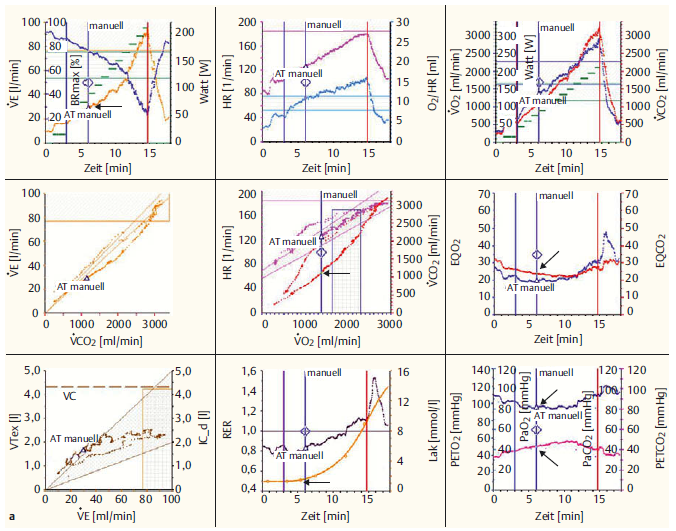
\includegraphics[width=7cm]{Bilder/9fieldcomplex.png}
\caption{Beispiel einer 9-Felder-Grafik nach einer Spiroergometrie mit einer jungen sportlichen Frau}
\end{figure}
\end{frame}

\begin{frame}{Spiroergometrie: 9-Felder-Grafik}
\begin{itemize}
\item grafisches Instrument der Spiroergometrie zum Vergleich vieler unterschiedlicher Messwerte
\item Nummerierung von oben links nach unten rechts von eins bis neun
\item kann je nach diagnostischem Schwerpunkt sehr komplex werden
\item in der Sportmedizin sind nur bestimmte Felder relevant: Fokus auf Feld 4, 5, 6 und 9 (Scharhag-Rosenberger, 2013)
\item Grafik muss auf Darstellung der ventilatorischen Schwellen reduziert werden
\item mehrere existente Methoden zur Schwellenbestimmung
\end{itemize}
\end{frame}

\begin{frame}{Spiroergometrie: Methoden zur Schwellenbestimmung}
\begin{itemize}
\item wissenschaftlich renommierteste Methoden wurden von AG Spiroergometrie zusammengefasst (Westhoff et al., 2012)
\item zwei Methoden für jede Schwelle werden in dieser Arbeit untersucht
\end{itemize}
\begin{columns}
\begin{column}[t]{5cm}
\begin{block}{VT1}
\begin{enumerate}
\item V-Slope: erster überproportionaler Anstieg der \vcotwo{} gegenüber der \votwo
\item alleiniger Anstieg des Sauerstoff-Äquivalents \eqotwo
\end{enumerate}
\end{block}
\end{column}
\begin{column}[t]{5cm}
\begin{block}{VT2}
\begin{enumerate}
\item überproportionaler Anstieg der \ve{} gegenüber der \vcotwo
\item Anstieg des Kohlenstoffdioxid-Äquivalents \eqcotwo
\end{enumerate}
\end{block}
\end{column}
\end{columns}
\end{frame}

\begin{frame}{Spiroergometrie: Bestimmung der VT1}
\begin{columns}
\begin{column}{5cm}
\begin{figure}[H]
\begin{center}
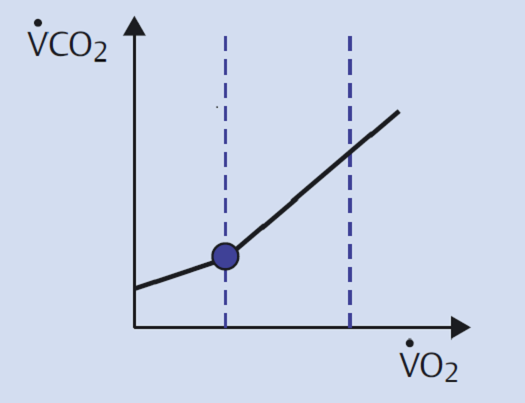
\includegraphics[width=40mm]{Bilder/vslope.png}
\caption{Schematische Darstellung der V-Slope-Methode}
\end{center}
\end{figure}
\end{column}
\begin{column}{5cm}
\begin{figure}[H]
\begin{center}
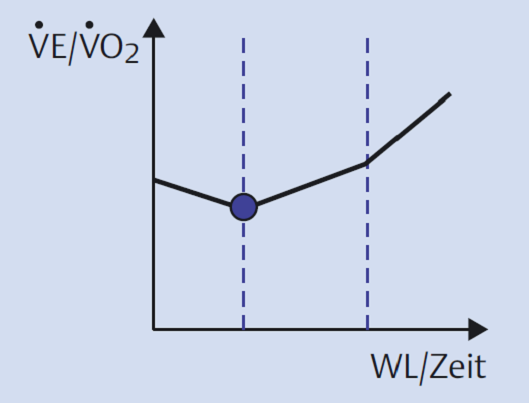
\includegraphics[width=40mm]{Bilder/eqo2.png}
\caption{Schematische Darstellung des \eqotwo}
\end{center}
\end{figure}
\end{column}
\end{columns}
\end{frame}

\begin{frame}{Spiroergometrie: Bestimmung der VT1}
\begin{columns}
\begin{column}[t]{5cm}
\begin{block}{V-Slope}
	\begin{itemize}
		\item grafischer Vergleich der \vcotwo{} und \votwo
		\item Identifizierung charakteristischer Knickpunkte in der Steigung (engl: \textsl{slope})
	\end{itemize}
\end{block}
\end{column}
\begin{column}[t]{5cm}
\begin{block}{\eqotwo}
	\begin{itemize}
		\item grafischer Vergleich des Verhältnisses aus \ve{} und \votwo{} zur Zeit in \si{\minute} oder Leistung in \si{\watt}
		\item Tiefpunkt der \eqotwo-Kurve = POW (Hollmann, 1958) = VT1
	\end{itemize}
\end{block}
\end{column}
\end{columns}
\end{frame}

\begin{frame}{Spiroergometrie: Bestimmung der VT2}
\begin{columns}
	\begin{column}{5cm}
		\begin{figure}[H]
			\begin{center}
				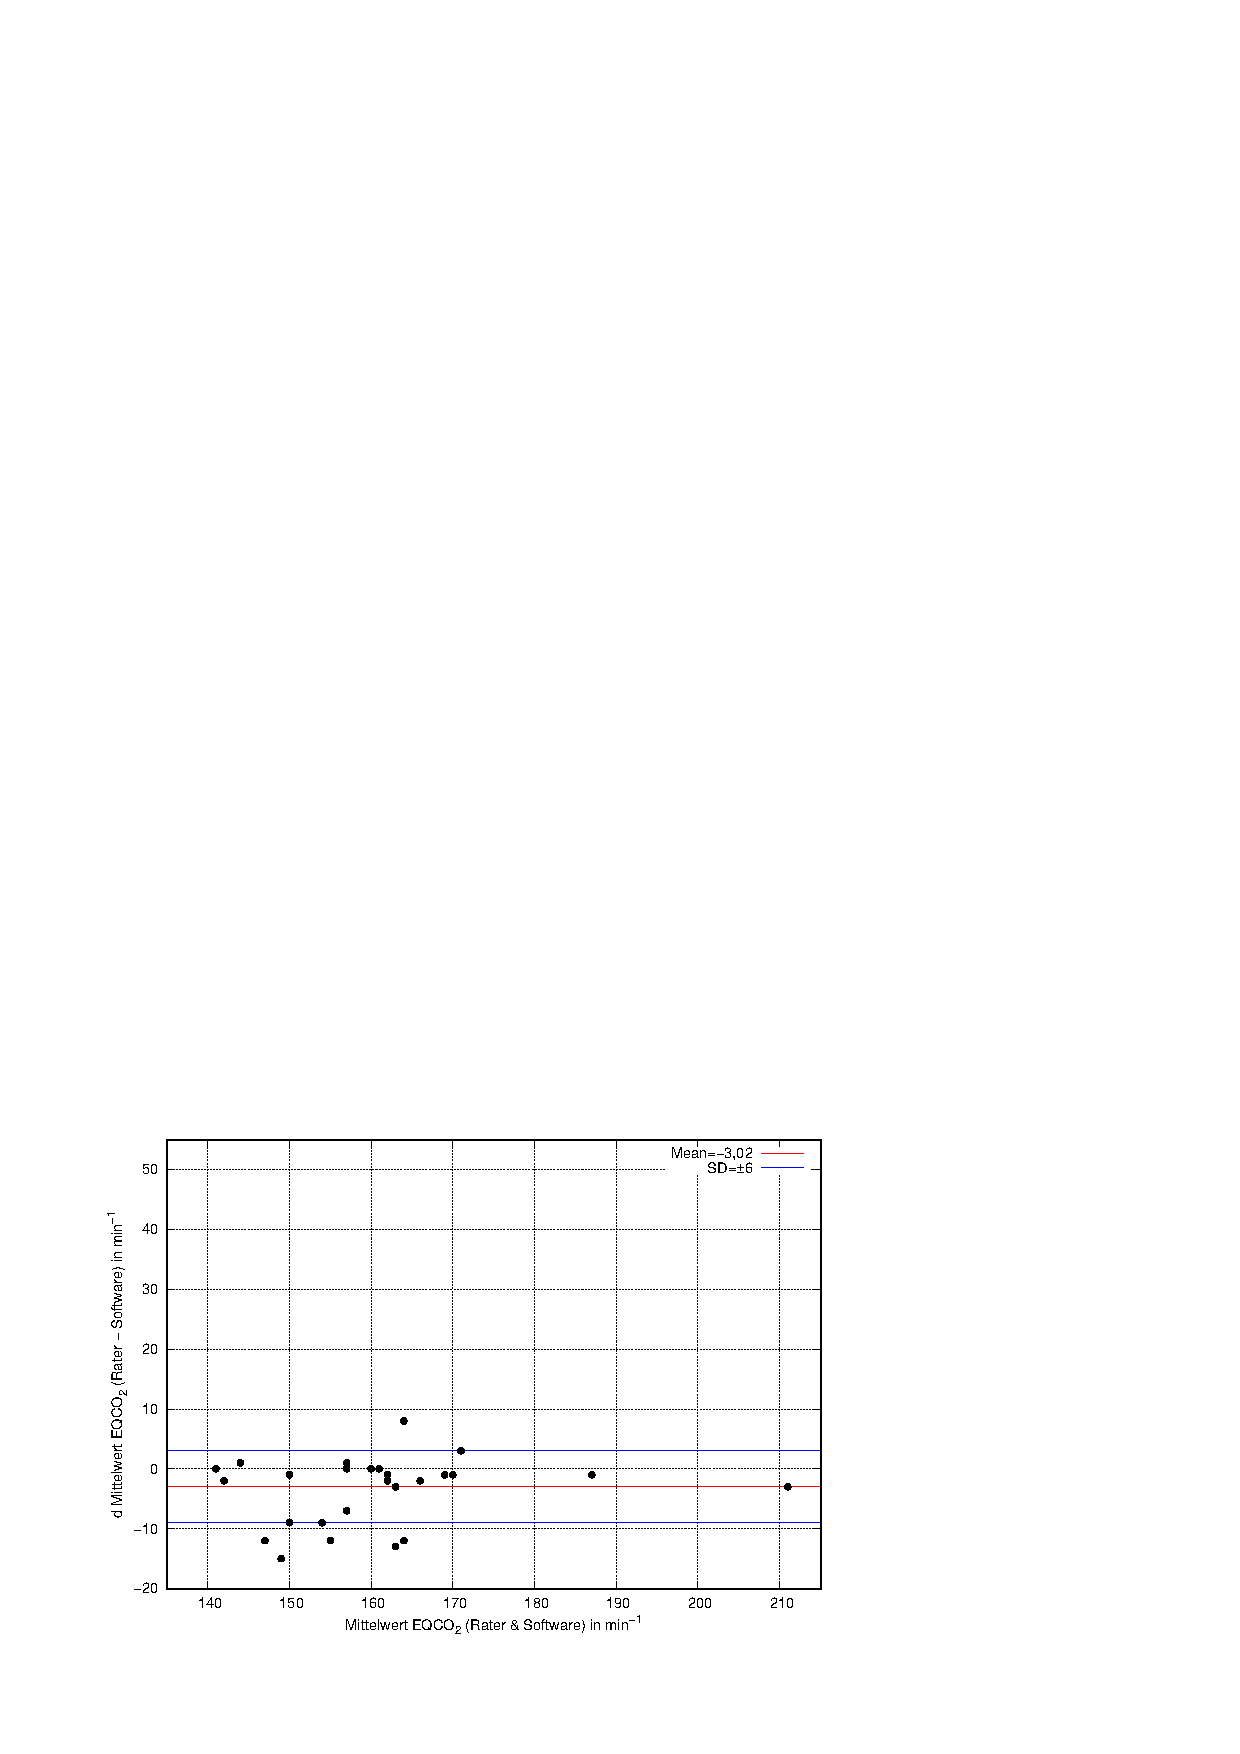
\includegraphics[width=40mm]{Bilder/eqco2.png}
				\caption{Schematische Darstellung des EQCO\textsubscript{2}}
			\end{center}
		\end{figure}
	\end{column}
	\begin{column}{5cm}
		\begin{figure}[H]
			\begin{center}
				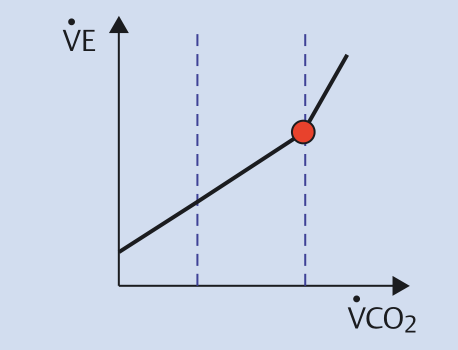
\includegraphics[width=40mm]{Bilder/field4.png}
				\caption{Schematische Darstellung von $\dot{V}E/\dot{V}CO_2$} 
			\end{center}
		\end{figure}
	\end{column}
\end{columns}
\end{frame}

\begin{frame}{Spiroergometrie: Bestimmung der VT2}
\begin{columns}
	\begin{column}[t]{5cm}
		\begin{block}{\eqcotwo}
			\begin{itemize}
				\item grafischer Vergleich des Verhältnisses aus \ve{} und \vcotwo{} zur Zeit in \si{\minute} oder Leistung in \si{\watt}
				\item charakteristische "`Badewannenform"'
				\item Anstieg der Kurve = VT2
			\end{itemize}
		\end{block}
	\end{column}
	\begin{column}[t]{5cm}
		\begin{block}{\ve/\vcotwo}
			\begin{itemize}
				\item grafischer Vergleich der \ve{} und \vcotwo{}, Analogie zum V-Slope
				\item überproportionale Steigungszunahme = VT2
			\end{itemize}
		\end{block}
	\end{column}
\end{columns}
\end{frame}

\begin{frame}{Fazit zur Problemstellung}
\begin{itemize}
	\item RQ = 1 ist als Methode in Studien umstritten
	\item RQ = 1 ist beeinflussbar (z.B. durch Ernährung)
	\item RQ = 1 wird unzureichend bei muskulärer Erschöpfung
	\item CCPS muss mit einem neuen und besseren Algorithmus optimiert werden
	\item vier alternative Methoden zur Bestimmung der VT1 und VT2 sind zu untersuchen
\end{itemize}
\end{frame}

\begin{frame}{Ziele der Arbeit}
\begin{block}{Forschungsfragen}
\begin{enumerate}
	\item Eignet sich der metabolicscan zur Durchführung der Spiroergometrie?
	\item Mit welcher Methode können die Schwellen optimal bestimmt werden?
	\item Ist eine genauere Bestimmung der VT2 mit den neuen Methoden möglich?
\end{enumerate}
\end{block}
\end{frame}
% -----------------------------------------------------------
% Kapitel 2: Methoden
% -----------------------------------------------------------
\section{Methoden}

\begin{frame}{Testprojekt}
\begin{itemize}
	\item spiroergometrische Testmessungen mit 28 internen und externen Probanden
	\item Personen zwischen 18 und 60 Jahren
	\item Sportler und Nicht-Sportler
	\item Raucher sowie Nichtraucher
	\item Messwerterfassung zur grafischen Auswertung mittels ausgewählter Methoden zur Schwellenbestimmung
\end{itemize}
\end{frame}

\begin{frame}{Material \& Testaufbau}
\begin{itemize}
	\item Laptop mit CCPS + angebundenes Ergometer der Firma \textsl{Emotion Fitness}
	\item zur vorangehenden Abklärung der kardialen Gesundheit: \textsl{cardioscan cs-3 effect} für Ruhe-EKG
	\item kalibriertes Modell des metabolicscan
	\item für jeden Probanden ein unbenutzter antibakterieller Polypropylen-Filter + flexibles Elastomer-Mundstück
\end{itemize}
\end{frame}

\begin{frame}{Funktionsweise des metabolicscan}
\begin{itemize}
	\item Modularer Aufbau: Atemmodul + Analysemodul
	\item Atemmodul enthält einen Flowsensor
	\item Messung der Strömungsgeschwindigkeit der Inspirations- und Exspirationsluft
	\item Berechnung des Strömungsvolumens durch mathematische Integration über die Zeit
	\item Analysemodul enthält CO\textsubscript{2}/O\textsubscript{2}-Sensormodul
	\item Pumpe saugt Luftanteil durch Probenschlauch zur Analyseeinheit
	\item CO\textsubscript{2}-Messung durch Infratotlichtabsorption
	\item Weiterleitung zum galvanischen O\textsubscript{2}-Sensor
\end{itemize}
\end{frame}

\begin{frame}{Aufbau des metabolicscan}
\begin{figure}[H]
	\centering
	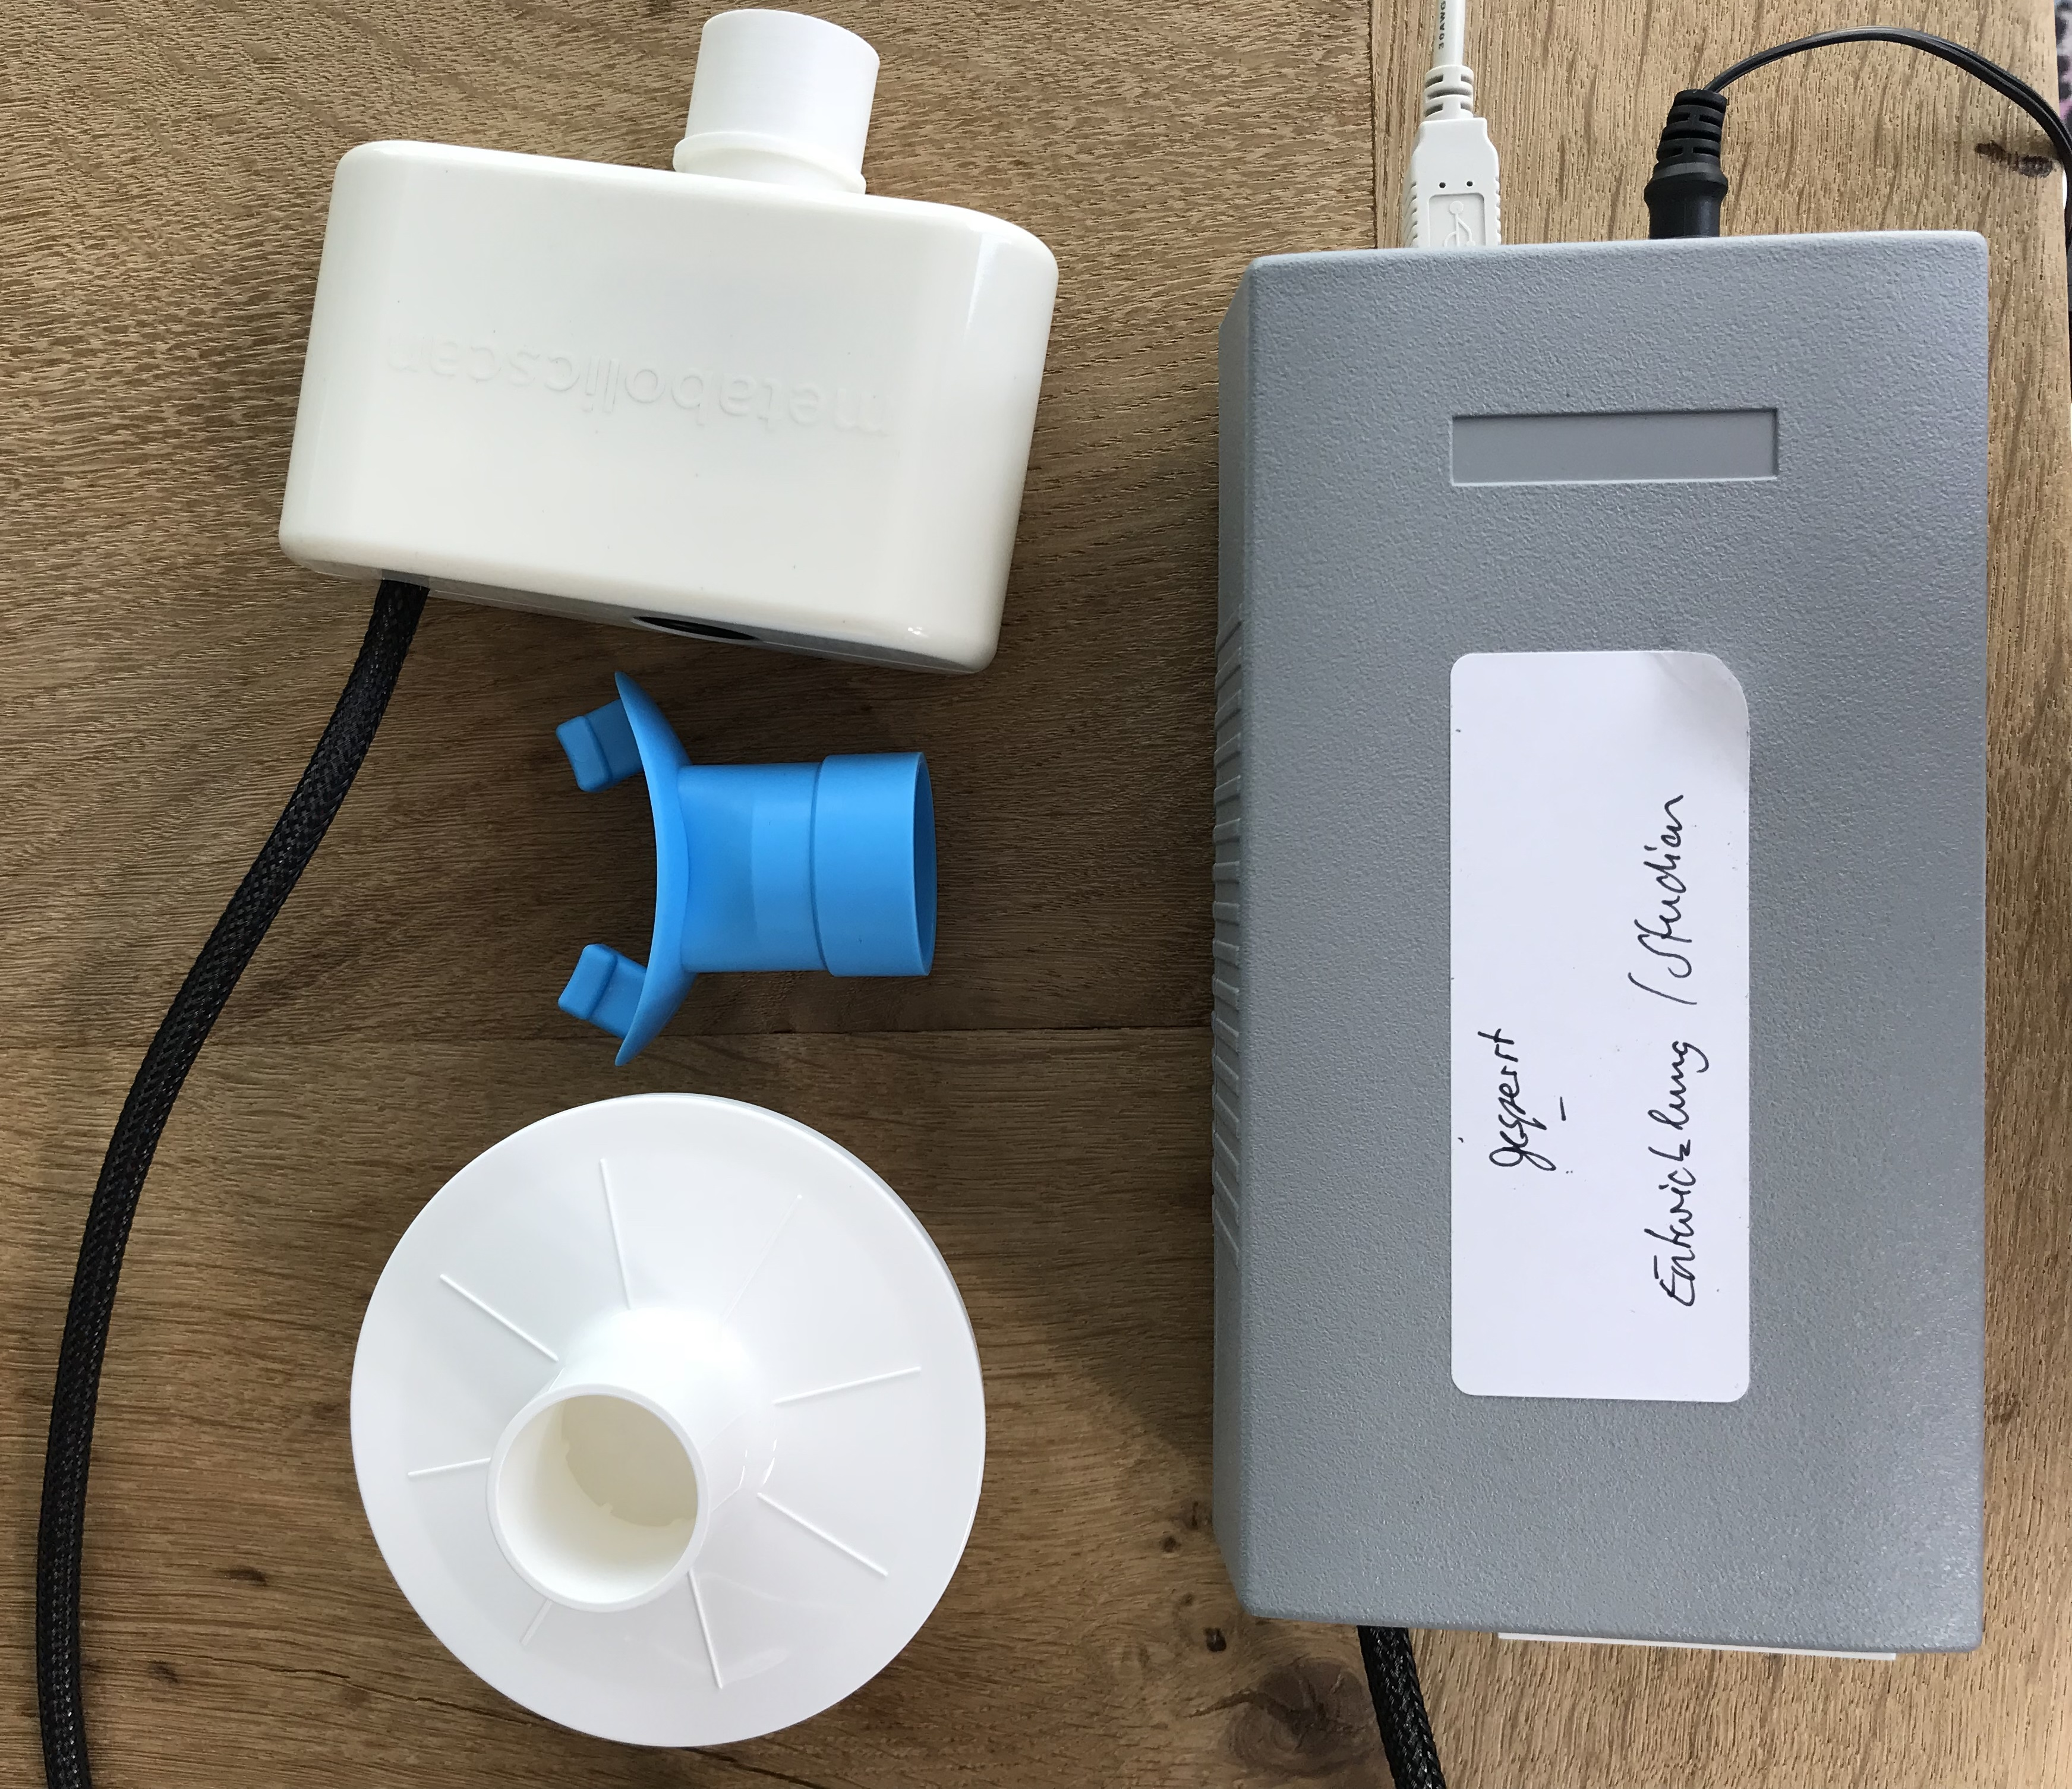
\includegraphics[width=7cm]{Bilder/mbs.jpg}
	\caption{metabolicscan: Analyseeinheit (rechts), Atemmodul (oben links), Filter (unten links) und Mundstück (blau)}
\end{figure}
\end{frame}

\begin{frame}{Messbedingungen}
\begin{itemize}
	\item alle Messungen im selben Raum
	\item Raumtemperatur zwischen \SI{18}{\degreeCelsius} und \SI{22}{\degreeCelsius}
	\item vor jeder Messung Belüftung des Raumes zur Minimierung des CO\textsubscript{2}-Anteils der Luft
	\item Ausschlusskriterien: akute fiebrige Infekte, Herz-Kreislauf-Erkrankungen, chronische Atemwegserkrankungen und Schwangerschaft
	\item keine anstrengenden Sporteinheiten am Vortag
	\item zwei Stunden vor der Messung keine Mahlzeiten/kein Koffein mehr
	\item gleichbleibende Trittfrequenz während der Messung
\end{itemize}
\end{frame}

\begin{frame}{Vorbereitung einer Messung}
\begin{itemize}
	\item Risikoabklärung + Anamnesebericht
	\item Ermittelung von Körpergewicht und Körpergröße
	\item Abklärung des Trainings- und Gesundheitszustandes
	\item zweiminütiger Herz-Stress-Test mit cardioscan
	\item Anlegen des Pulsgurtes zur HF-Überwachung während der Messung
	\item Justierung des Ergometer-Sattels
	\item Berechnung der maximalen Soll-Leistung in \si{\watt} mittels zweier Formeln (Jones und SHIP)
	\item Bestimmung des individuellen Belastungsprotokolls nach WHO- oder BAL-Schema (abhängig vom Trainingszustand)
\end{itemize}
\end{frame}

\begin{frame}{Abbruchkriterien}
\begin{itemize}
	\item fallende HF trotz zunehmender Belastung
	\item allgemeine Herzbeschwerden, Engegefühl in der Brust
	\item Atemnot
	\item auffällige Blässe
	\item akute Kopfschmerzen
	\item Schwindel oder Sehstörungen
	\item starke subjektive Erschöpfung
	\item Beinschwäche oder Muskelkrämpfe
	\item andauernder Abfall der Trittfrequenz
\end{itemize}
\end{frame}

\end{document}